% Hi! We're member of IRIS-HEP and the Scikit-HEP community project, where we are building
% a Pythonic data analysis ecosystem for HEP community.
% IRIS-HEP does lots of things from data delivery, to cyberinfrastructure, and supporting the
% development of existing software tools, and has been a community center for fostering Scikit-HEP
% development.
% A shared goal is that we want to empower analysts at the LHC and beyond with modern data science stacks
% and build powerful libraries that allow for analysts to build expressive analysis workflows.
\begin{frame}{Hello from IRIS-HEP and Scikit-HEP!}
  \begin{columns}
    \column{0.6\textwidth}
    \Large
    % \begin{itemize}
    \begin{itemize}\setlength{\itemsep}{0.5 cm}
      \item We're members of the \href{https://iris-hep.org/}{Institute for Research and Innovation in Software for High Energy Physics (IRIS-HEP)} and the \href{https://scikit-hep.org/}{Scikit-HEP} community project developing a Pythonic data analysis ecosystem for HEP
      \item Goals: Empower analysts with modern data science stacks and provide powerful libraries for building expressive workflows
    \end{itemize}
%
    \column{0.4\textwidth}
    \begin{figure}
        \begin{center}
            \href{https://iris-hep.org/}{
\includegraphics[width=0.9\linewidth]{iris-hep-logo-long.pdf}}
            \href{https://scikit-hep.org/}{
\includegraphics[width=0.8\linewidth]{scikit-hep-logo.pdf}}
        \end{center}
    \end{figure}
  \end{columns}
\end{frame}

% Given that we're at the "Python exchange" we're not going to do a "Why Python" slide
% as we don't need to convert the choir, but what we can do it tell you a bit about how our
% community went from being C++ only to a 2 language C++ and Python community.
% This plot shows a survey that Jim Pivarski did of **users** of the code in the CMS experiment's (one of the main experiments at the
% Large Hadron Collider) software framework monorepo "CMSSW" which is publicly available on GitHub.
% He cross referenced the people who forked CMSSW (so filtering on particle physicists on CMS) and then searched _their_
% repositories for "import" statements in files.
% As we can see, before 2018 most of these imports were coming from C++.
% However, around 2018 we see a change where Python is becoming the dominant form of code that is actually being written
% by these users (both as scripts and in Jupyter).
\begin{frame}{Rapid rise of Python for analysis in HEP}
\vspace{0.25 cm}
\textcolor{darkblue}{Source: ``\mintinline{python}{import XYZ}'' matches in GitHub repos for users who fork CMSSW.}

% If we take a more detailed view of this survey, we can see that this increase in people writing more Python is also
% strongly tied with the use of scientific Python packages in the HEP community, as we see with numpy, matplotlib, pandas,
% and tensorflow.
% This is also tied with the rise of Scikit-HEP which got started around 2017 and IRIS-HEP late 2018 / early 2019, which you
% can see also with the appearance of tooling that came out of IRIS-HEP and Scikit-HEP like uproot and awkward Array.
\vspace{0.2 cm}
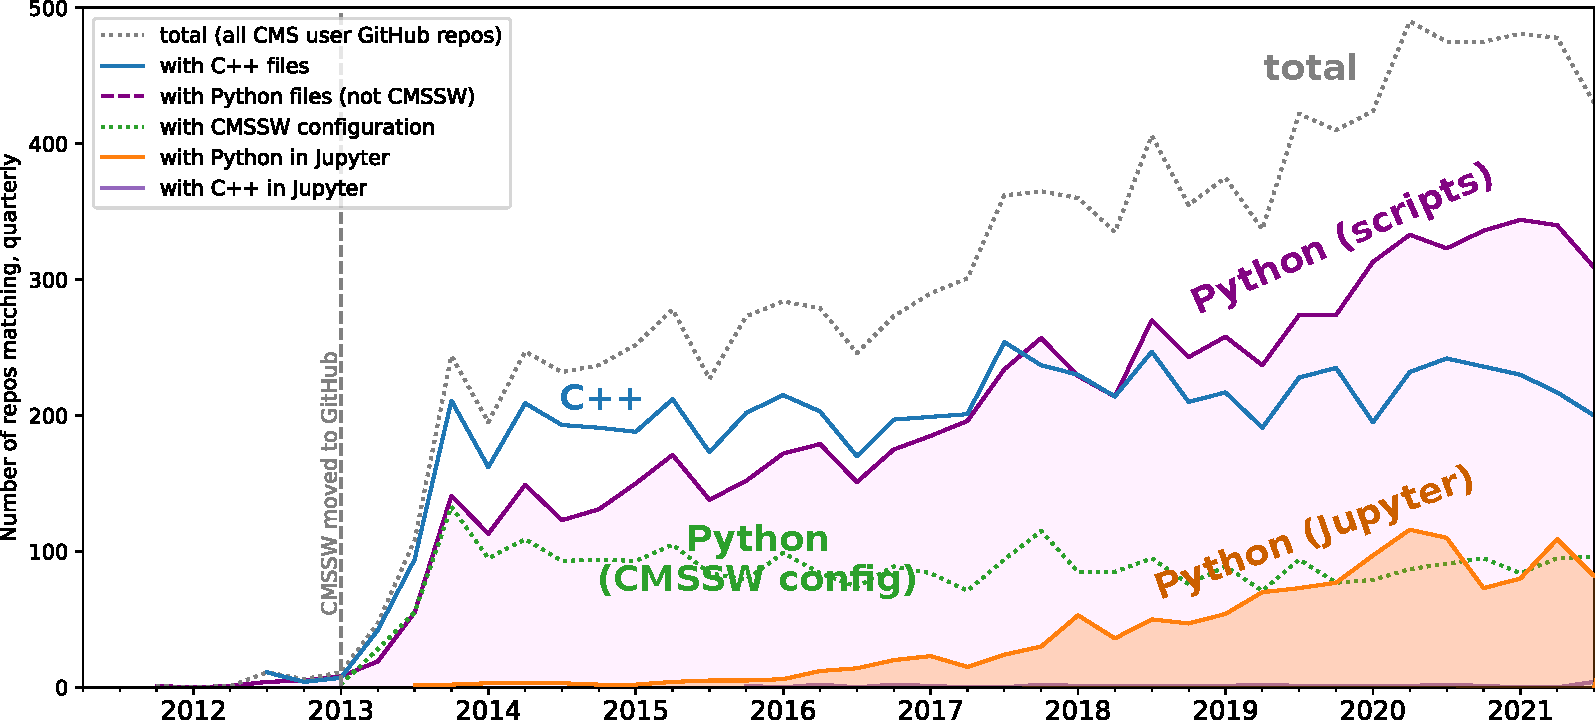
\includegraphics[width=\linewidth]{github-language-fullstudy-for-review.pdf}
\textcolor{darkblue}{\tiny (CMSSW is the CMS experiment's ``offline'' software framework)}
\end{frame}

\begin{frame}{Explosion of Scientific Python (NumPy, etc.) use recent since 2018}
\vspace{0.25 cm}
\textcolor{darkblue}{Source: ``\mintinline{python}{import XYZ}'' matches in GitHub repos for users who fork CMSSW.}

\vspace{0.2 cm}
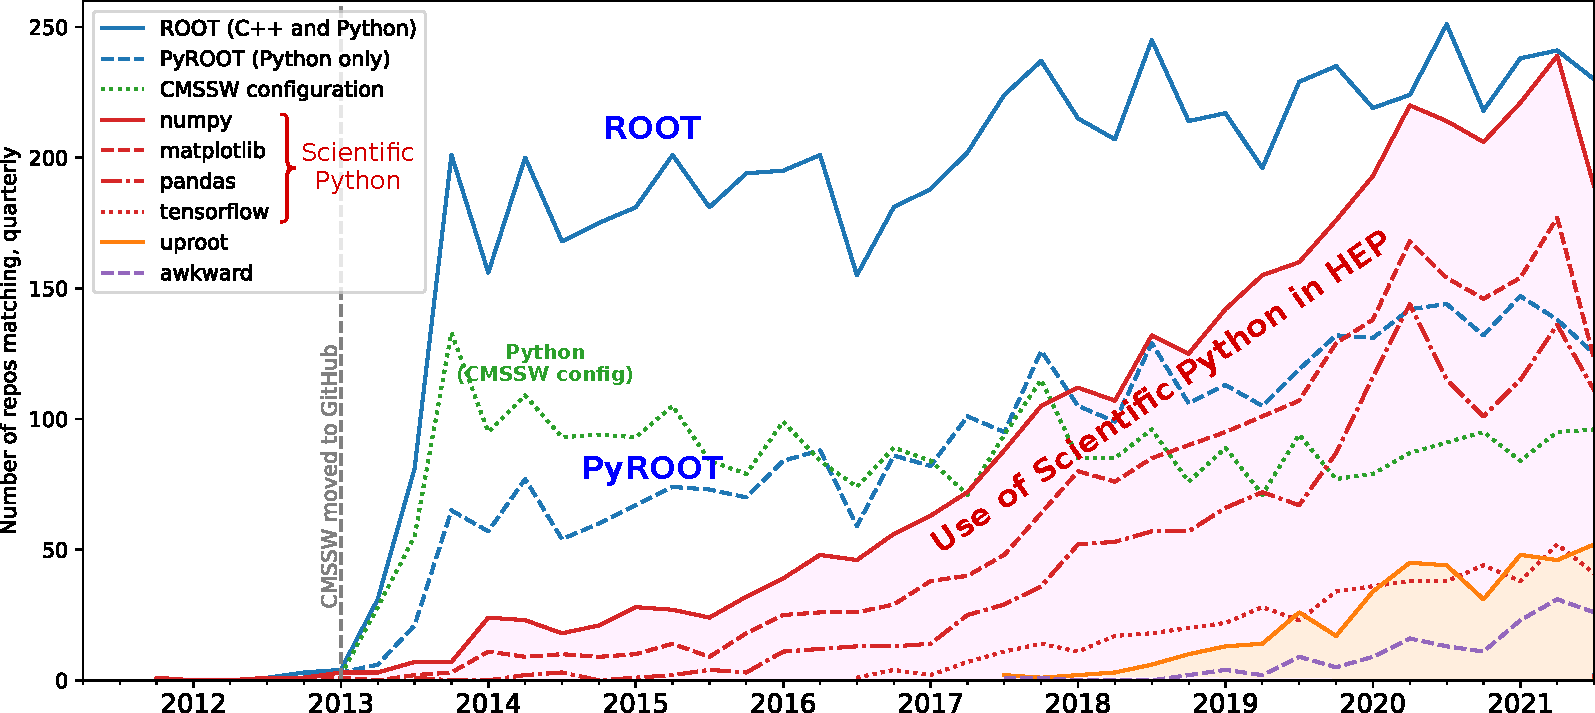
\includegraphics[width=\linewidth]{github-package-fullstudy-for-review.pdf}
\end{frame}

\begin{frame}{Growth tightly coupled to the rise of Scikit-HEP supported by IRIS-HEP}
\vspace{0.25 cm}
\textcolor{darkblue}{Source: ``\mintinline{bash}{pip install XYZ}'' download rate for MacOS/Windows (no batch jobs).}

\vspace{0.1 cm}
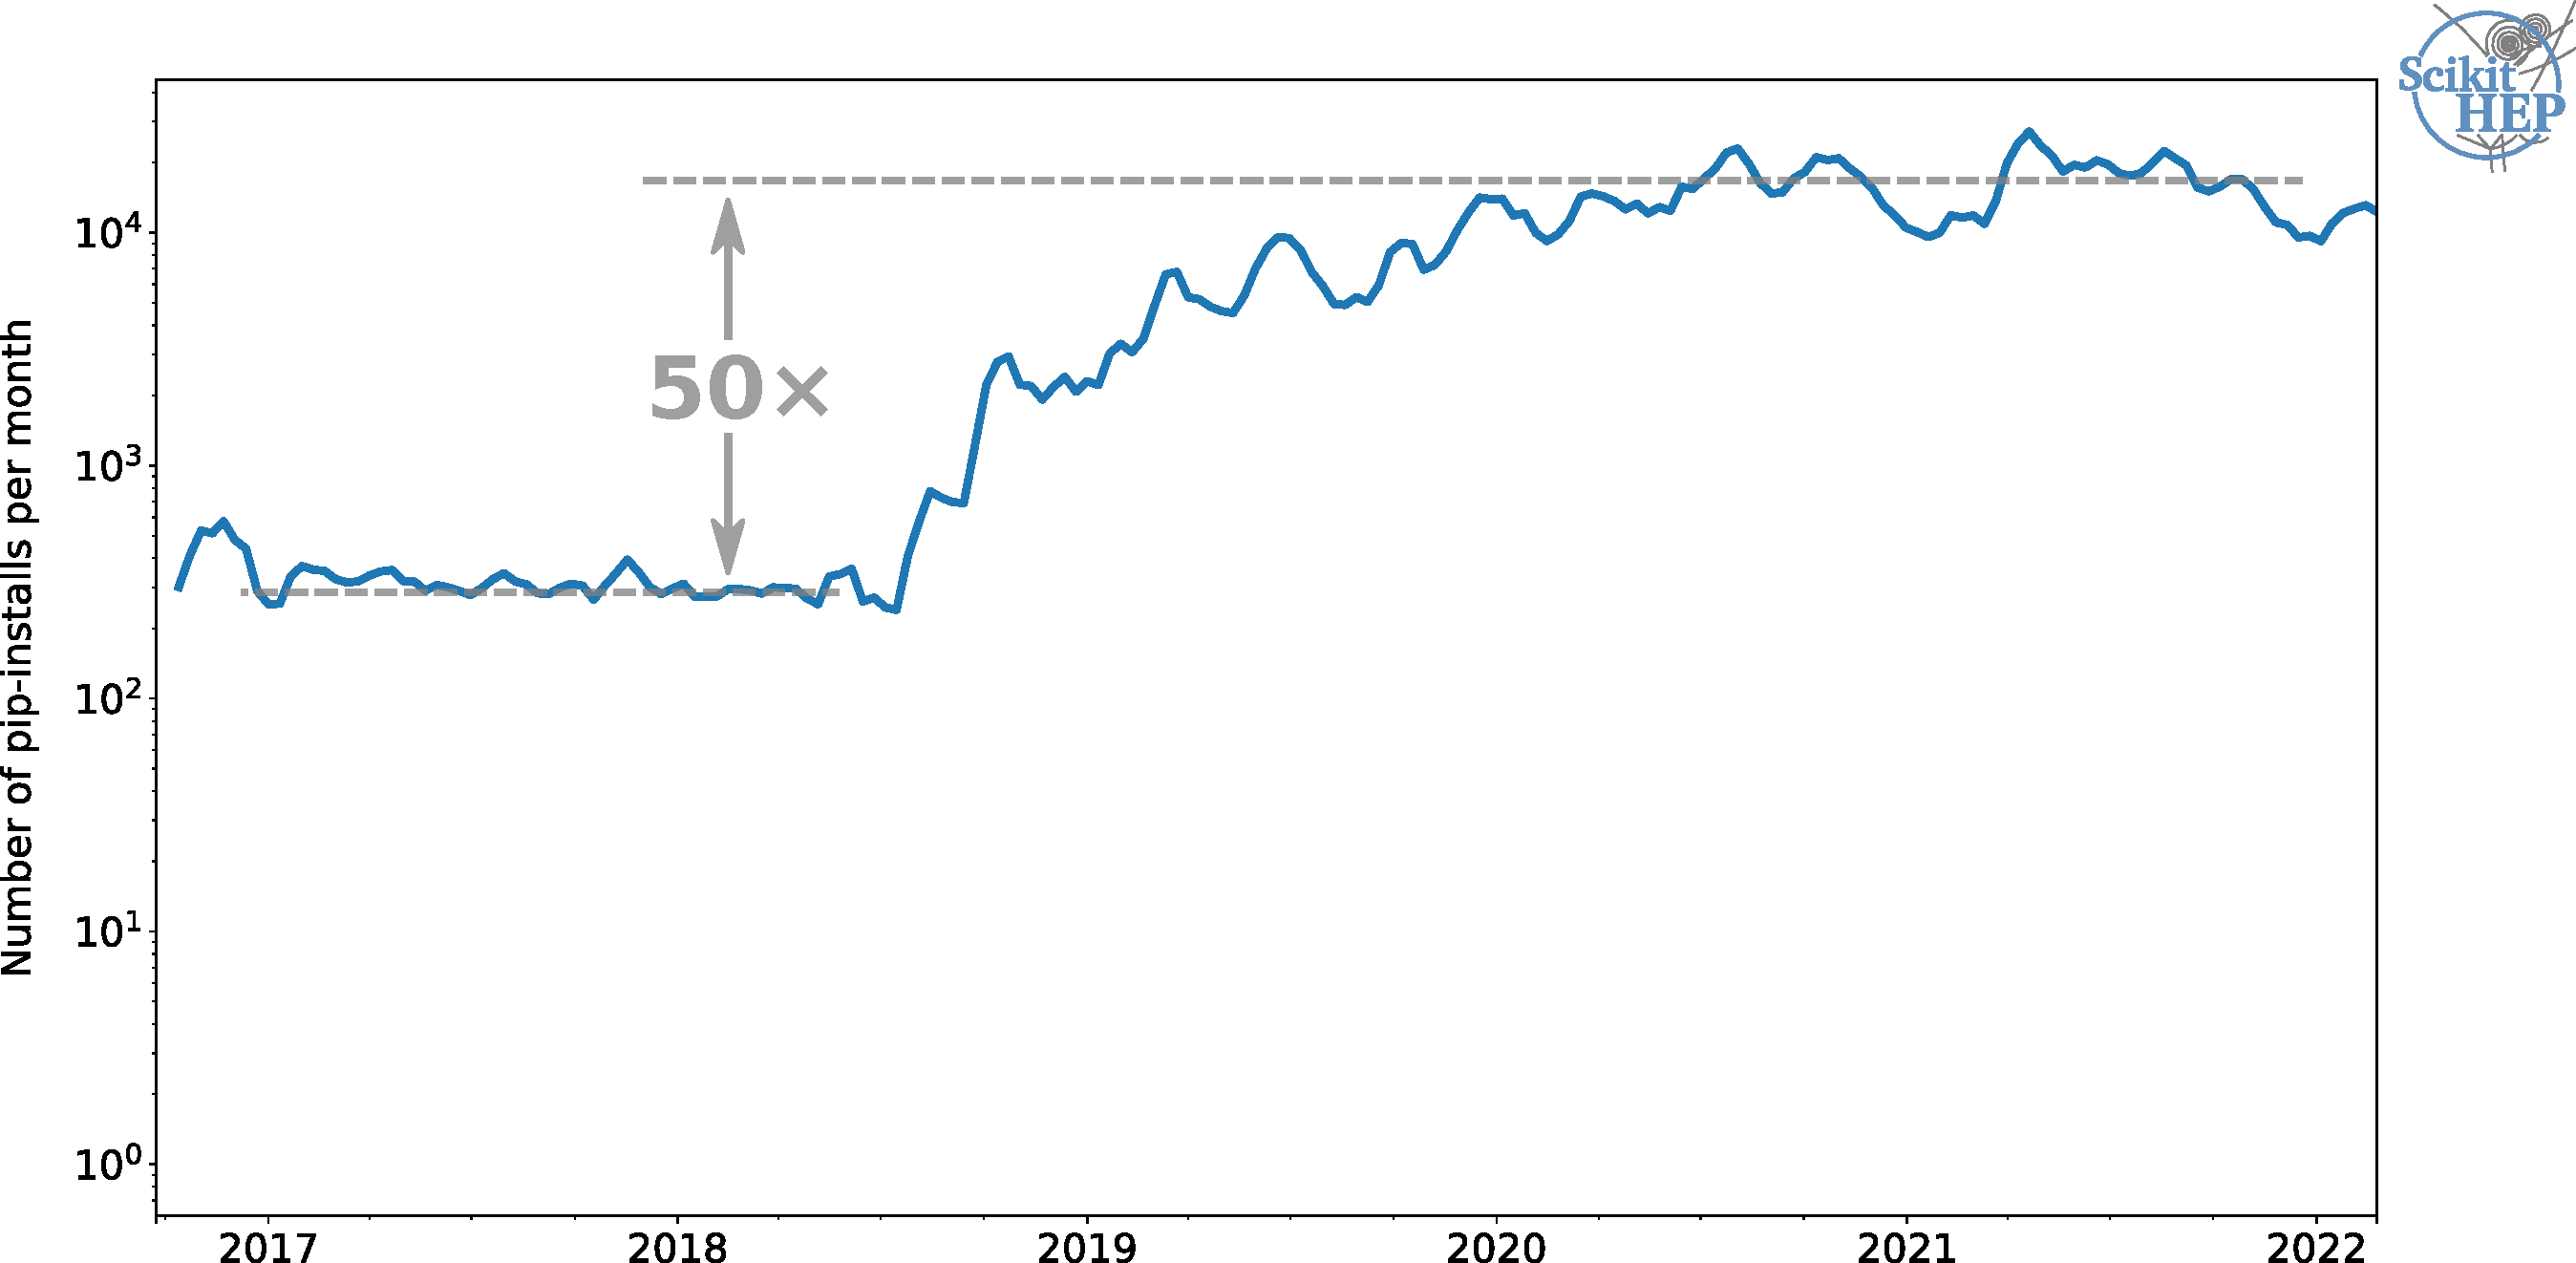
\includegraphics[width=\linewidth]{pip-macwin-scikithep-log-combined.pdf}
\end{frame}

\begin{frame}{Growth tightly coupled to the rise of Scikit-HEP supported by IRIS-HEP}
\vspace{0.25 cm}
\textcolor{darkblue}{Source: ``\mintinline{bash}{pip install XYZ}'' download rate for MacOS/Windows (no batch jobs).}

\vspace{0.1 cm}
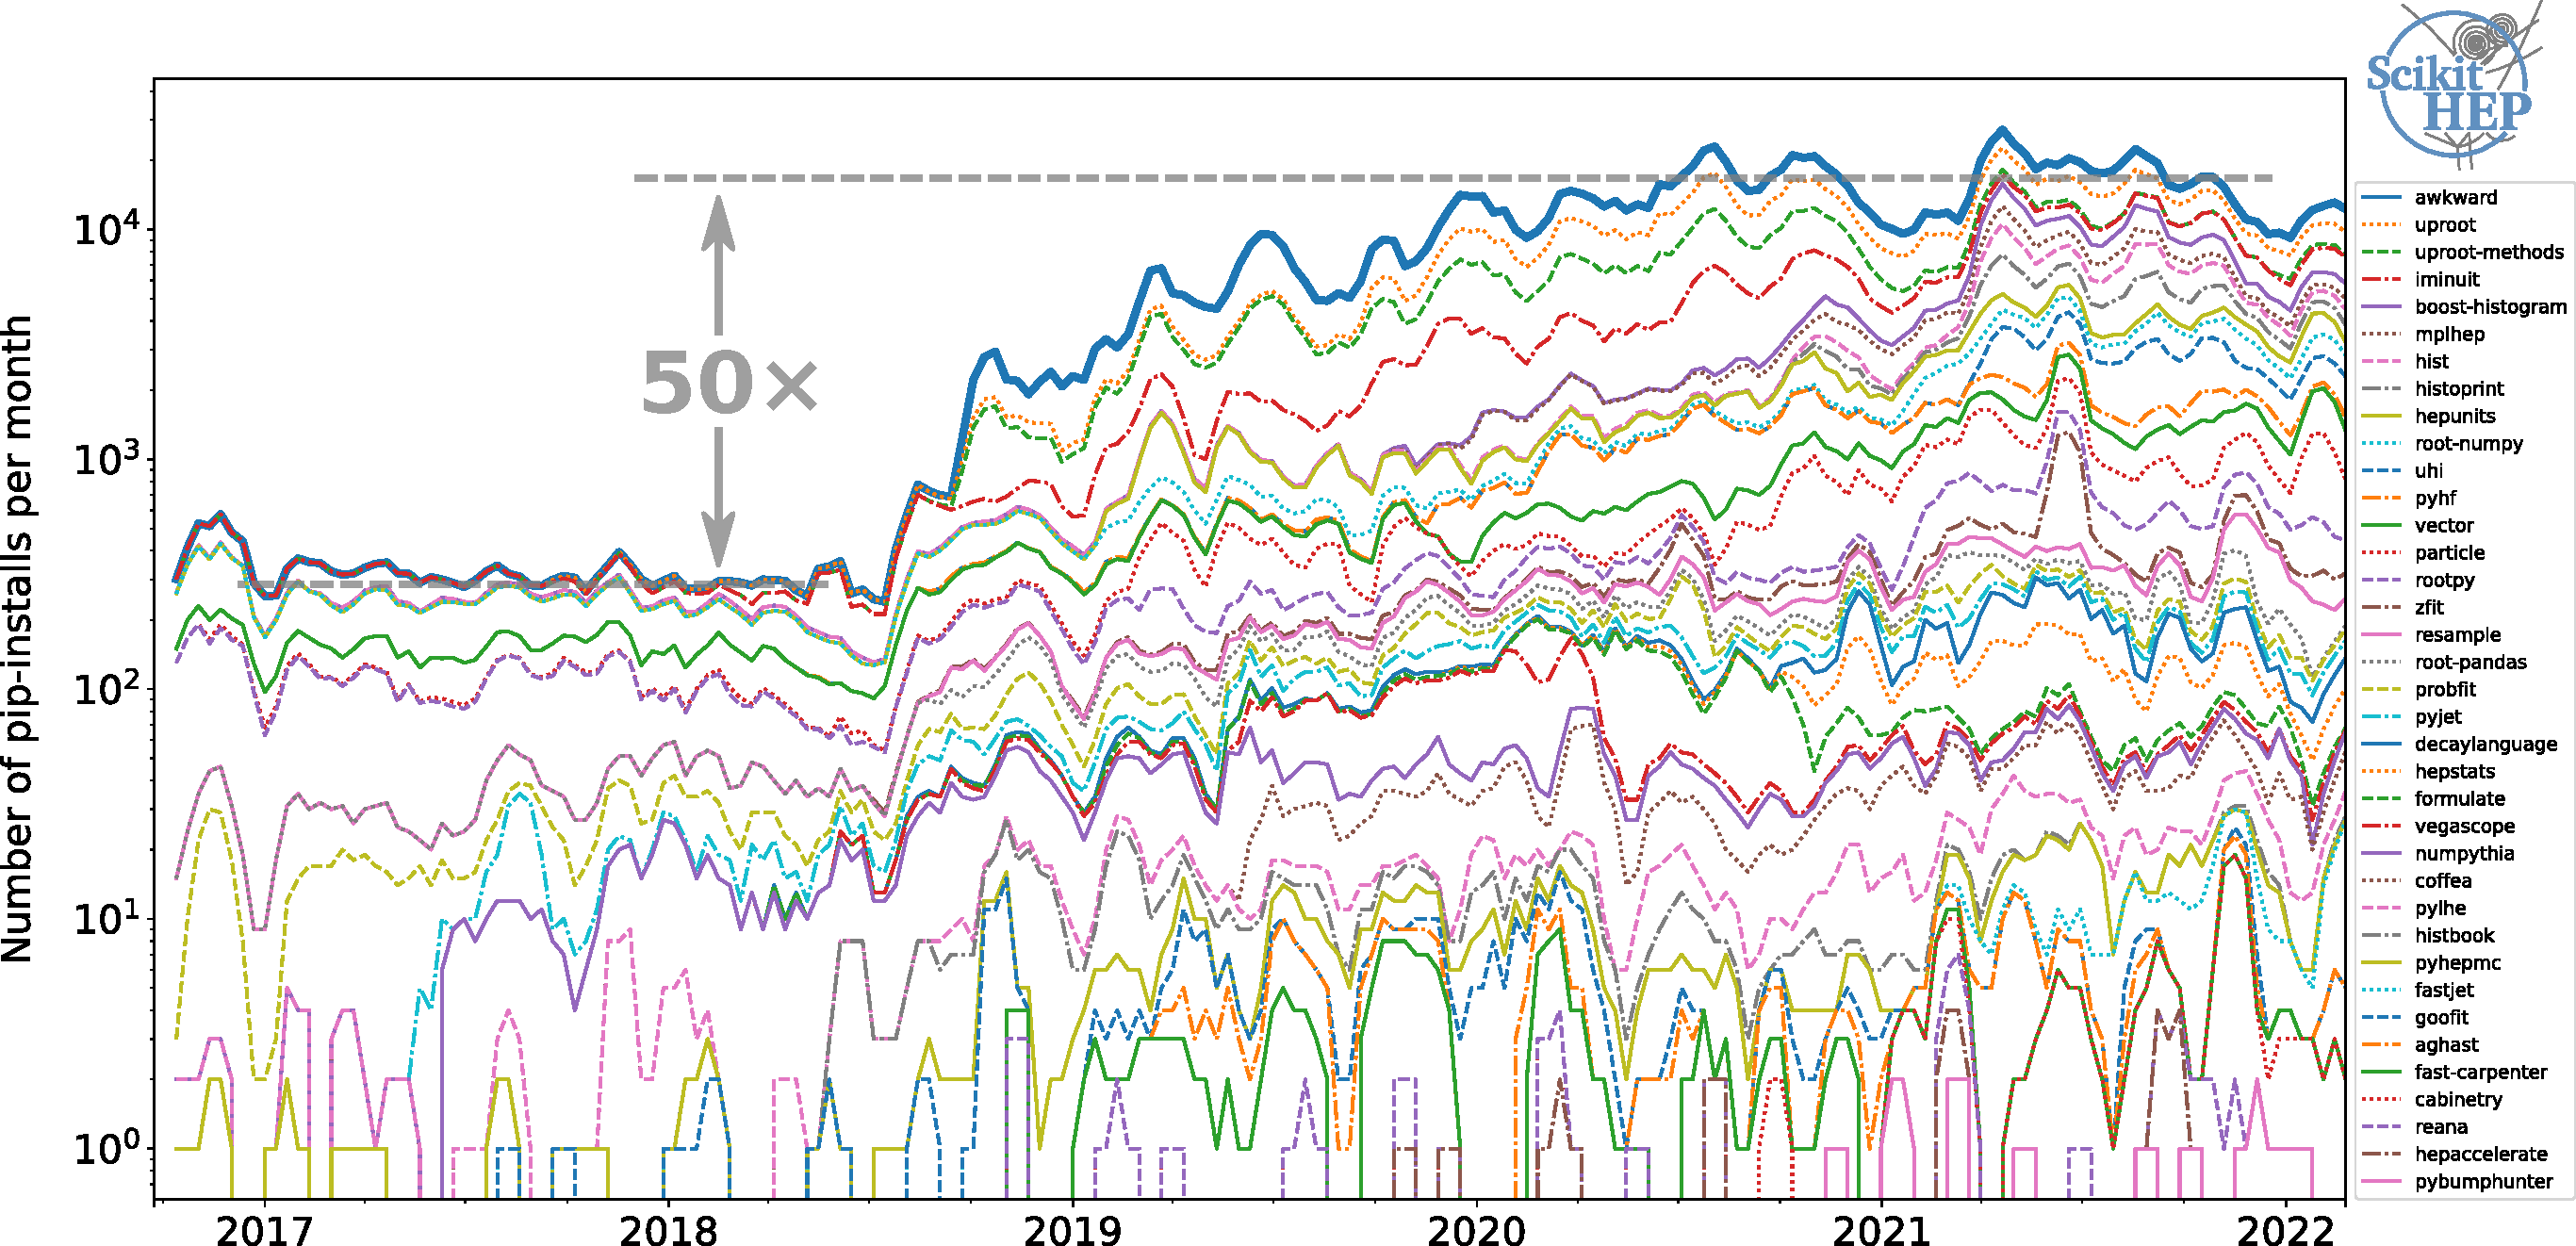
\includegraphics[width=\linewidth]{pip-macwin-scikithep-log-by-package.pdf}
\end{frame}

\begin{frame}{Ecosystems}
\vspace{0.25 cm}
\begin{center}
    {\small In his \href{https://youtu.be/ZyjCqQEUa8o}{PyCon 2017 keynote}, Jake VanderPlas gave us the iconic ``PyData ecosystem'' image}
\end{center}

\vspace{0.1 cm}
\begin{figure}
    \begin{center}
        \href{https://coiled.io/blog/pydata-dask/}{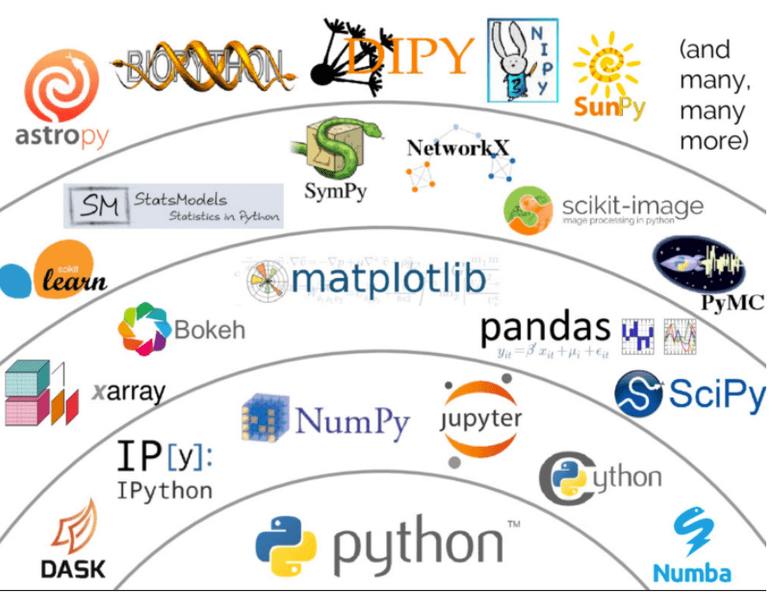
\includegraphics[width=0.60\linewidth]{pydata-ecosystem-pycon-2017.png}}
    \end{center}
\end{figure}
\end{frame}

\begin{frame}{Pythonic ecosystem for particle physics}
\vspace{0.25 cm}
\begin{center}
    {\small Working view of a PyHEP ecosystem (Scikit-HEP and IRIS-HEP supported projects)}
\end{center}

% \vspace{0.1 cm}
\begin{figure}
    \begin{center}
        \href{https://indico.cern.ch/event/1140031/}{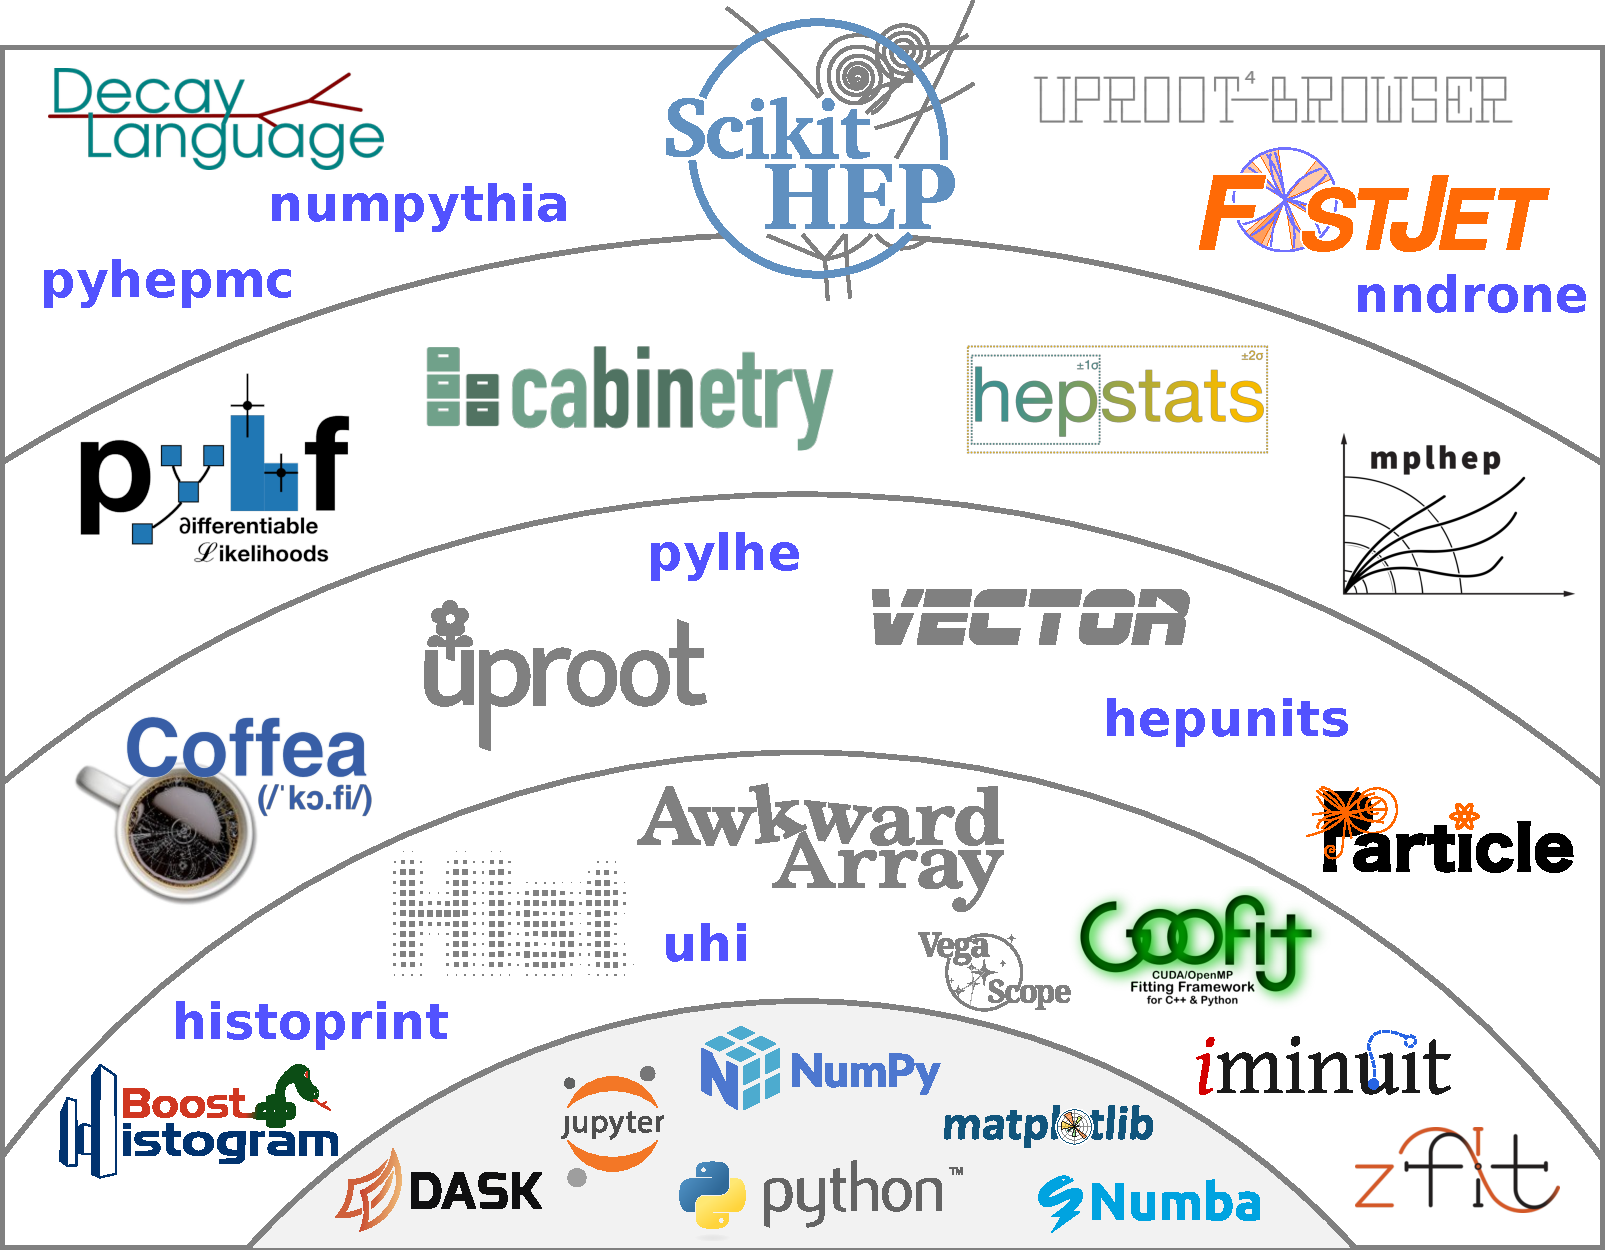
\includegraphics[width=0.60\linewidth]{shells-hep.pdf}}
    \end{center}
\end{figure}
\end{frame}

\begin{frame}{Built with intentionality and interoperability}
  \begin{columns}
    \column{0.45\textwidth}
    \begin{enumerate}\setlength{\itemsep}{0.5 cm}
      \item[5] HEP-specific UI applications or packaged algorithms
      \item[4] HEP-specific for common problems
      \item[3] HEP-specific, foundational
      \item[2] needed to create, but not really HEP-specific
      \item[1] non-HEP software we depend on
    \end{enumerate}
%
    \column{0.55\textwidth}
    \begin{figure}
        \begin{center}
            \href{https://indico.cern.ch/event/1140031/}{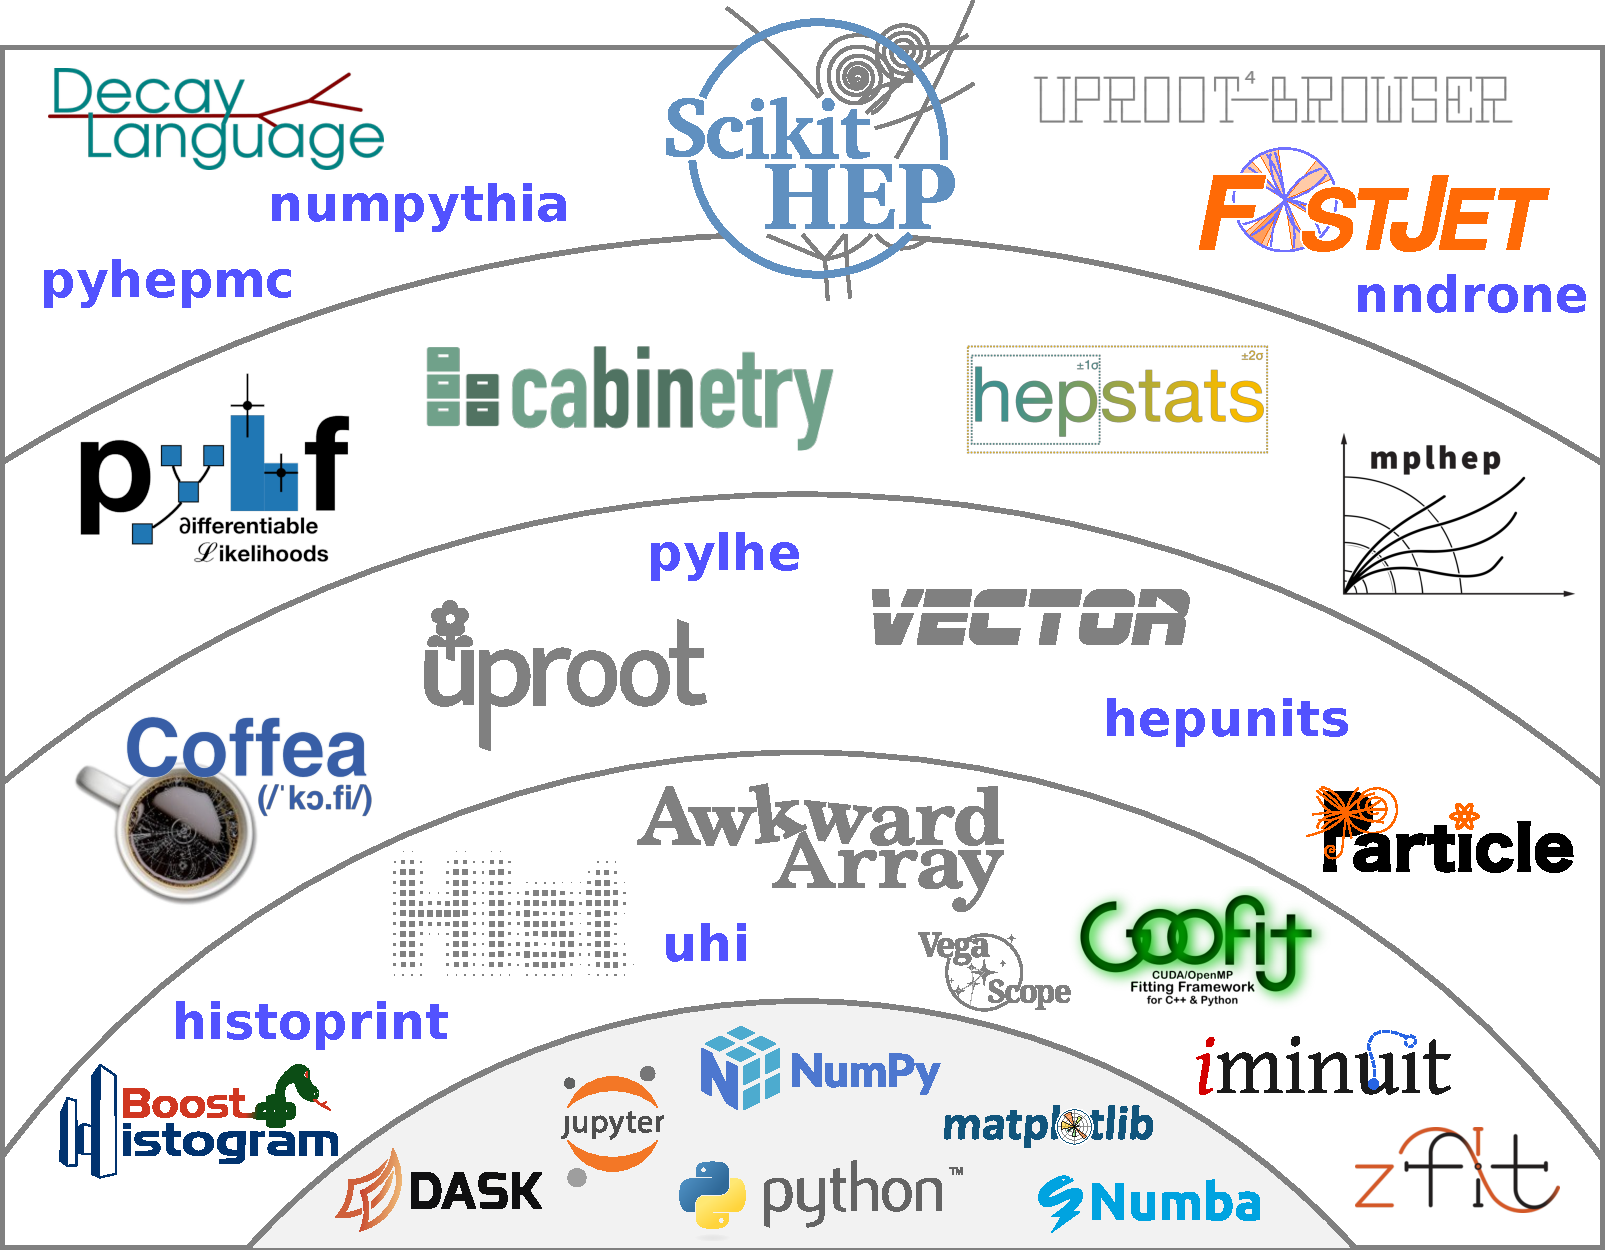
\includegraphics[width=\linewidth]{shells-hep.pdf}}
        \end{center}
    \end{figure}
  \end{columns}
\end{frame}
